%%%%%%%%%%%%%%%%%%%%%%%%%%%%%%%%%%%%%%%%%%  不使用 authblk 包制作标题  %%%%%%%%%%%%%%%%%%%%%%%%%%%%%%%%%%%%%%%%%%%%%%
%-------------------------------PPT Title-------------------------------------
\title{致敬民族脊梁,探索核武奥秘}
%\subtitle{两弹元勋与核弹原理}
%-----------------------------------------------------------------------------

%----------------------------Author & Date------------------------------------
%\author[]{\vskip +10pt 高朋林\inst{}} %[]{} (optional, use only with lots of authors)
%% - Give the names in the same order as the appear in the paper.
%% - Use the \inst{?} command only if the authors have different
%%   affiliation.
\institute[BCC]{\inst{}%
%\institute[Gain~Strong]{\inst{}%
\vskip -15pt 北京市计算中心}
%\vskip -20pt {\large 格致斯创~科技}}
\date[\today] % (optional, should be abbreviation of conference name)
{	%{\fontsize{6.2pt}{4.2pt}\selectfont{\textcolor{blue}{E-mail:~}\url{jiangjun@bcc.ac.cn}}}
\vskip 45 pt {\fontsize{8.2pt}{6.2pt}\selectfont{%清华大学\;\;物理系% 报告地点
	\vskip 5 pt \textrm{2025.04}}}
}

%% - Either use conference name or its abbreviation
%% - Not really information to the audience, more for people (including
%%   yourself) who are reading the slides onlin%%   yourself) who are reading the slides onlin%%   yourself) who are reading the slides onlineee
%%%%%%%%%%%%%%%%%%%%%%%%%%%%%%%%%%%%%%%%%%%%%%%%%%%%%%%%%%%%%%%%%%%%%%%%%%%%%%%%%%%%%%%%%%%%%%%%%%%%%%%%%%%%%%%%%%%%%

\subject{}
% This is only inserted into the PDF information catalog. Can be left
% out.
%\maketitle
\frame
{
%	\frametitle{\fontsize{9.5pt}{5.2pt}\selectfont{\textcolor{orange}{“高通量并发式材料计算算法与软件”年度检查}}}
\titlepage
}
%-----------------------------------------------------------------------------

%------------------------------------------------------------------------------列出全文 outline ---------------------------------------------------------------------------------
\section*{}
\frame[allowframebreaks]
{
	\frametitle{\textrm{Outline}}
%  \frametitle{\textcolor{mycolor}{\secname}}
  \tableofcontents%[current,currentsection,currentsubsection]
}
%在每个section之前列出全部Outline
%类似的在每个subsection之前列出全部Outline是\AtBeginSubsection[]
%\AtBeginSection[]
%{
%  \frame<handout:0>%[allowframebreaks]
%  {
%    \frametitle{Outline}
%%全部Outline中,本部分加亮
%    \tableofcontents[current,currentsection]
%  }
%}

%-----------------------------------------------PPT main Body------------------------------------------------------------------------------------
\small

% 幻灯片3:时代呼唤——两弹决策
\section{我国核武器的研制}
\begin{frame}
    \frametitle{时代呼唤——两弹决策}
\textrm{20}世纪中期,国际局势风云变幻,地缘政治错综复杂
\begin{itemize}
		\setlength{\itemsep}{8pt}
	\item ``冷战''持续:~朝鲜战争爆发后,新中国面临严峻的安全挑战
	\item 美、苏等国对核武器技术的垄断,对我国的国防构成巨大威胁
\end{itemize}
为了维护国家主权和安全,打破核垄断,党中央高瞻远瞩,果断作出研制原子弹、导弹的战略决策
%    \vspace{0.5cm}
    \begin{figure}
        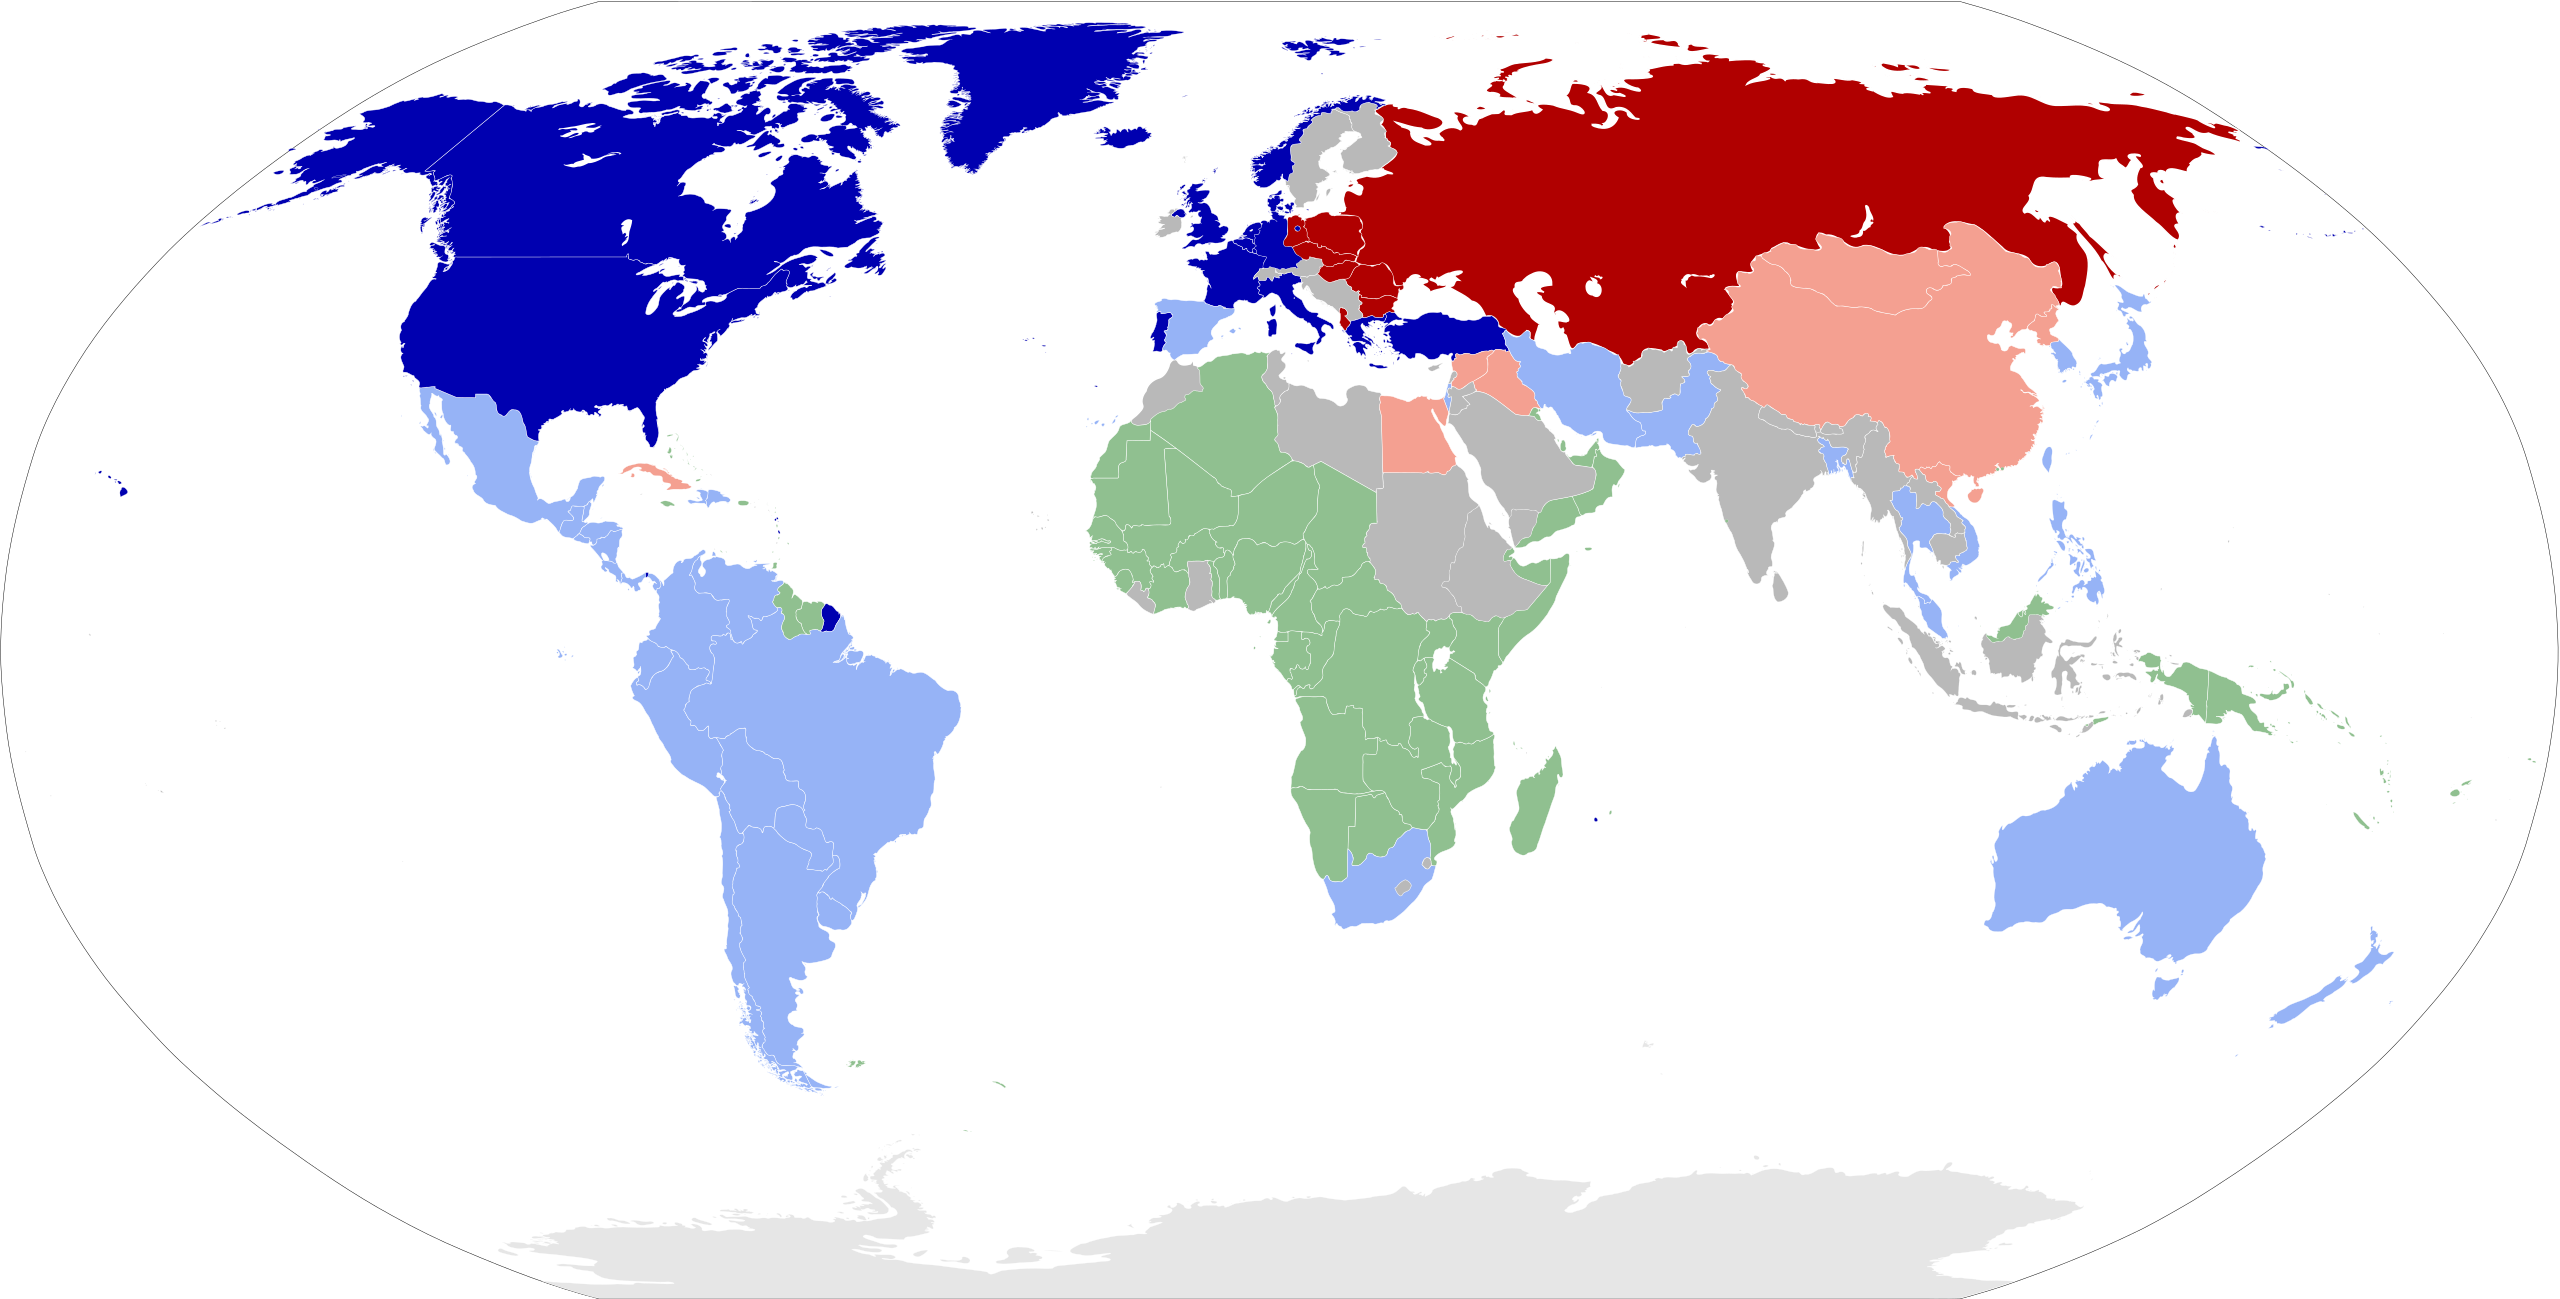
\includegraphics[width=0.8\textwidth]{Figures_History/Cold_War_Map-1959.png}
    \end{figure}
\end{frame}

\begin{frame}
    \frametitle{大漠孤烟——横空出世}
    \vspace{-0.4cm}
            \begin{figure}
                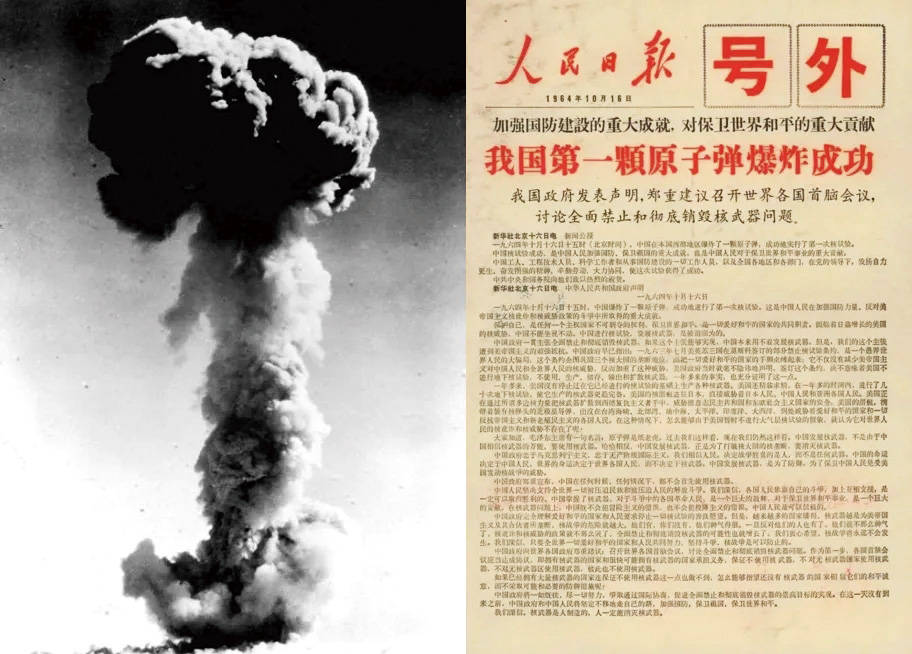
\includegraphics[width=0.95\textwidth]{Figures_History/People_Daily.jpeg}
%                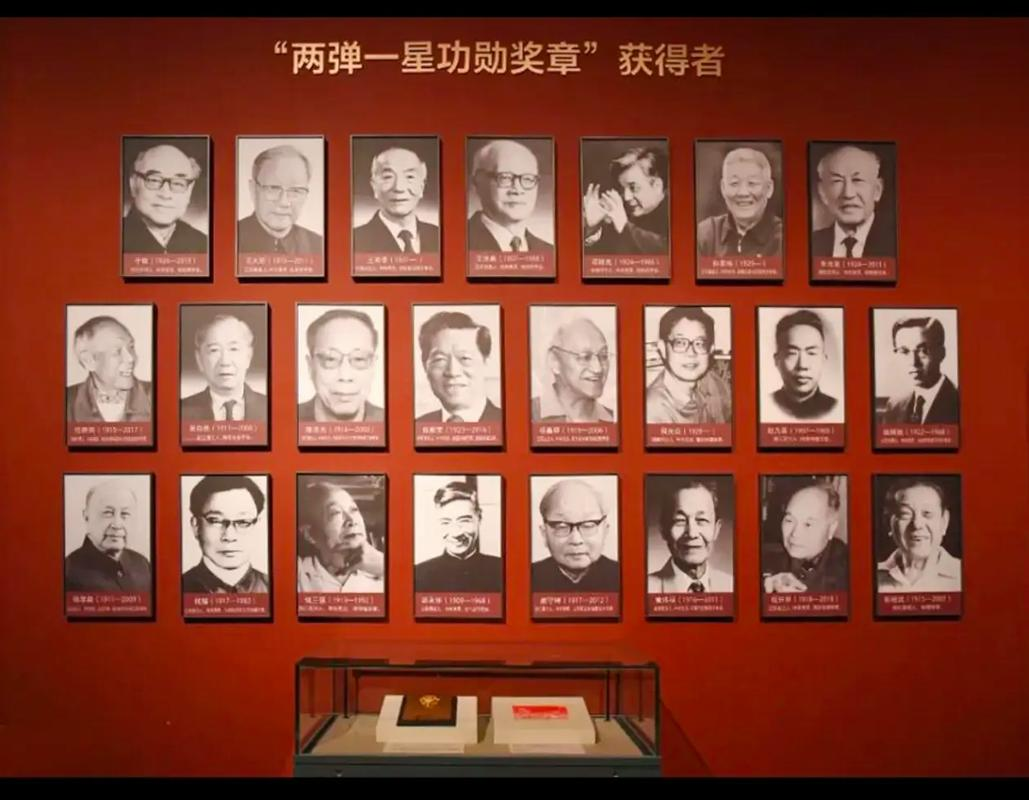
\includegraphics[width=0.95\textwidth]{Figures_History/Collection_23-1.jpeg}
		\caption{\tiny{\textrm{1964}年\textrm{10}月\textrm{16}日\textrm{15:00},我国第一颗原子弹爆炸成功}}
            \end{figure}
\end{frame}

\begin{frame}
    \frametitle{与日争辉——惊天动地}
    \vspace{-0.4cm}
            \begin{figure}
                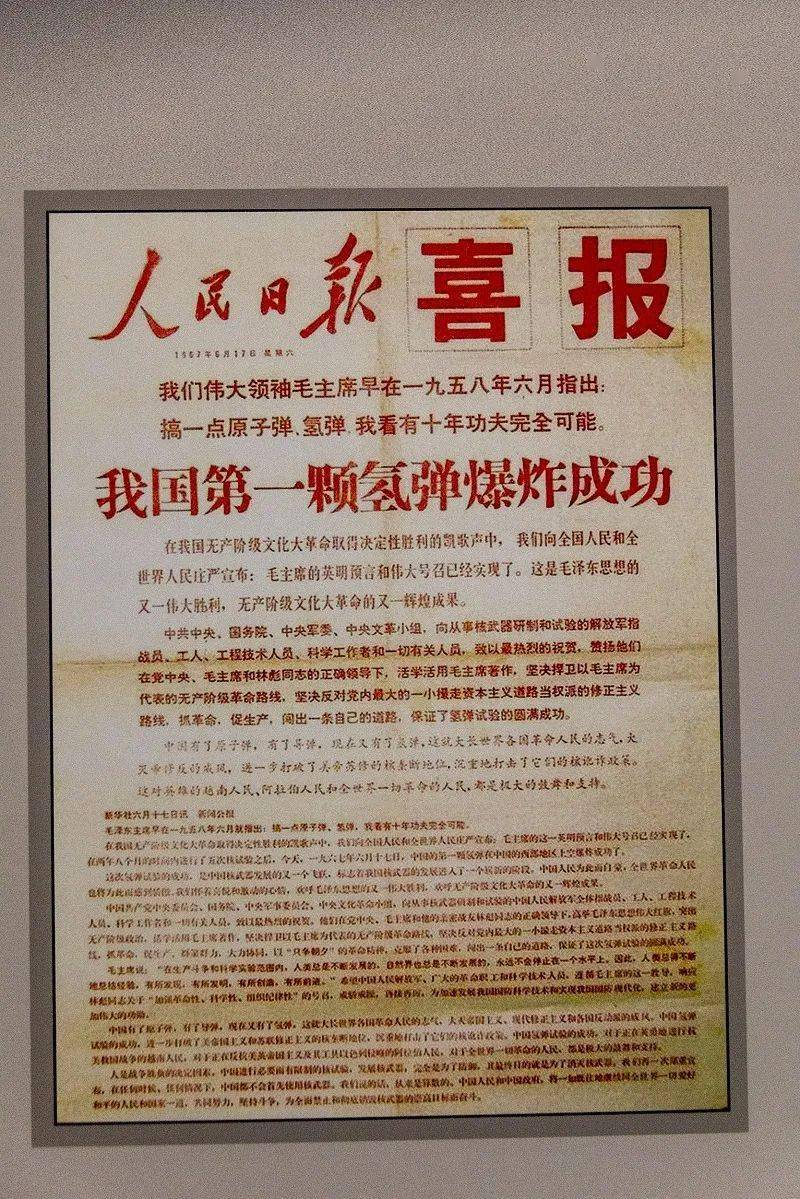
\includegraphics[width=0.53\textwidth, viewport=10 30 760 1000,clip]{Figures_History/People_Daily-2.jpeg}
%                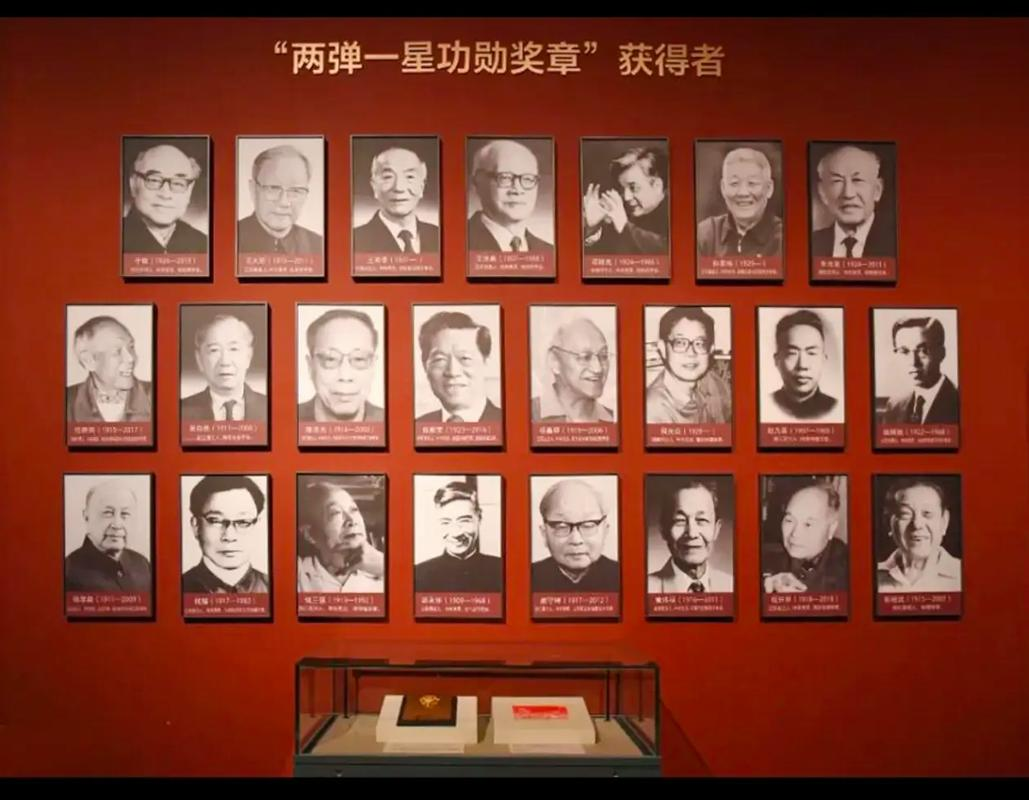
\includegraphics[width=0.95\textwidth]{Figures_History/Collection_23-1.jpeg}
		\caption{\tiny{\textrm{1967}年\textrm{6}月\textrm{17}日\textrm{8:20},我国第一颗氢弹爆炸成功}}
            \end{figure}
\end{frame}

\begin{frame}
    \frametitle{核弹模型}
            \begin{figure}
                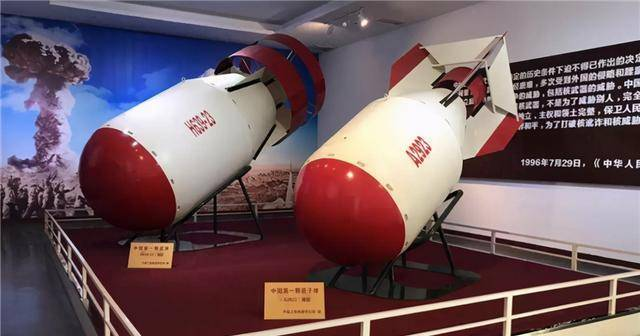
\includegraphics[width=0.95\textwidth]{Figures_History/Model.jpeg}
		\caption{\tiny{我国爆炸的第一颗原子弹和氢弹模型\textrm(1:1)}}
            \end{figure}
\end{frame}

% 幻灯片4:民族脊梁——两弹元勋
\begin{frame}
    \frametitle{民族脊梁——``两弹一星''元勋}
%    \begin{columns}[T]
%        \column{0.3\textwidth}
%            \begin{figure}
%                \includegraphics[width=\textwidth]{dengjiaxian.jpg}
%                \caption{邓稼先}
%            \end{figure}
%        \column{0.7\textwidth}
%            邓稼先不顾辐射危险,深入实验一线,为我国核武器事业奉献一生。
%    \end{columns}
%    \begin{columns}[T]
%        \column{0.3\textwidth}
%            \begin{figure}
%                \includegraphics[width=\textwidth]{qiansen.jpg}
%                \caption{钱学森}
%            \end{figure}
%        \column{0.7\textwidth}
%            钱学森冲破重重阻力,毅然回国,为我国导弹和航天事业奠定基础 。
%    \end{columns}
    \vspace{-0.4cm}
            \begin{figure}
                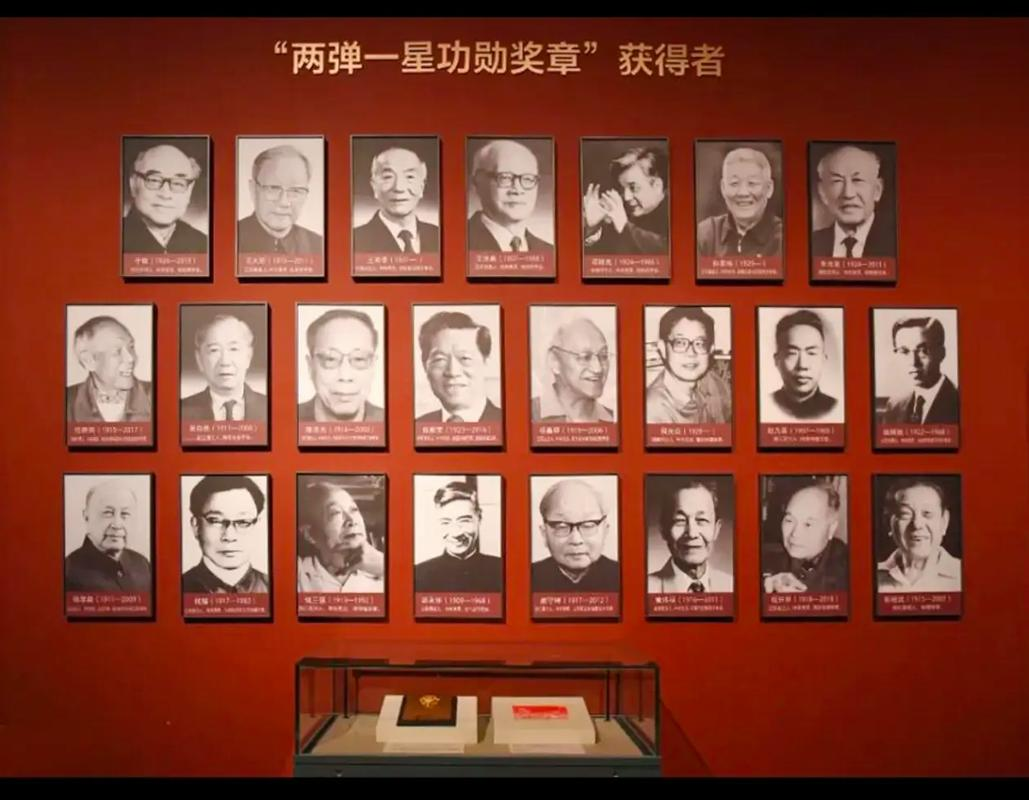
\includegraphics[width=0.95\textwidth]{Figures_History/Collection_23-1.jpeg}
		\caption{\tiny{\textrm{1999}年中央表彰的``两弹一星''功勋科学家}}
            \end{figure}
\end{frame}

% 幻灯片5:裂变之火——原子弹原理
\section{原子弹的原理、构造与引爆}
\begin{frame}
    \frametitle{裂变之火——原子弹原理}
%    \textbf{核裂变}
    \vskip -0.4cm
    \begin{figure}
        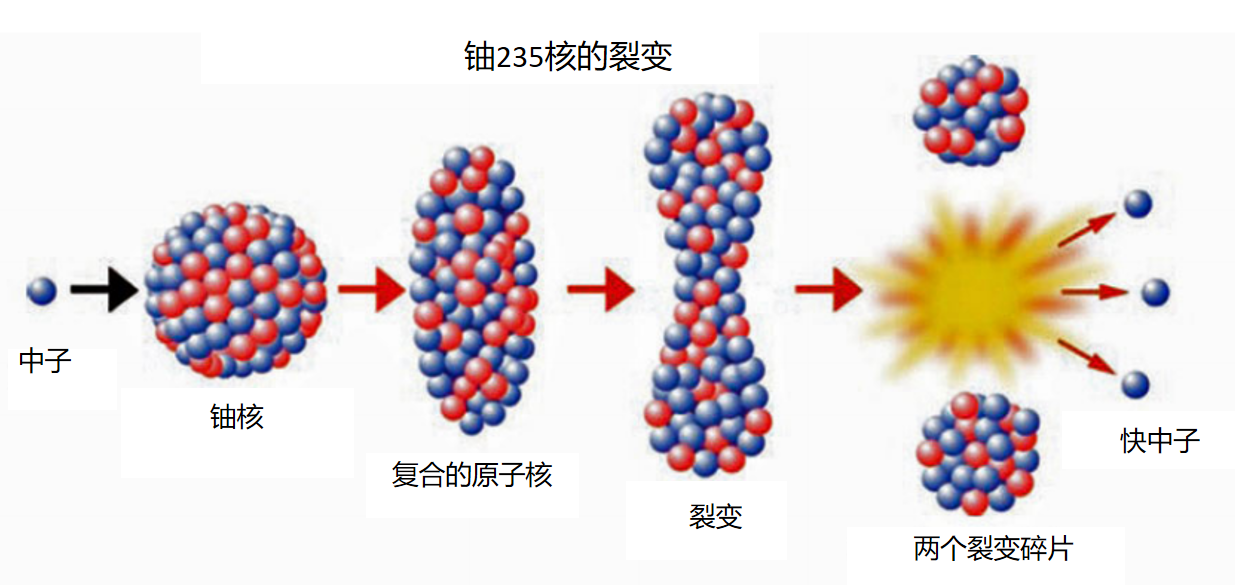
\includegraphics[width=0.72\textwidth]{Figures_History/Nuclear-energy-U235.png}
    \end{figure}
    \begin{itemize}
	    \item 裂变原理:~当重原子核{\fontsize{7.2pt}{6.2pt}\selectfont{~(如$\mathrm{U}^{235}$与$\mathrm{Pu}^{239}$)}},受到中子轰击时,会分裂成两个或多个较轻的原子核\\
		    {\fontsize{7.2pt}{6.2pt}\selectfont{以$\mathrm{U}^{235}$为例,被中子轰击后,会分裂成$\mathrm{Kr}^{92}$和$\mathrm{Ba}^{141}$,并释放$2\sim3$个中子和大量能量,裂变反应可表示为:
		    \begin{displaymath}
			    ^{235}_{92}\mathrm{U} + ^{1}_{0}n \rightarrow ^{92}_{36}\mathrm{Kr} + ^{141}_{56}\mathrm{Ba} + 2 - 3^{1}_{0}n + \mathrm{energy}
		    \end{displaymath}}}
        \item 链式反应:~裂变释放的中子,获得足够的动能继续轰击其他重原子核,可能引发持续的核裂变过程\\
		{\fontsize{7.2pt}{6.2pt}\selectfont{当重核元素体积小于临界体积时,每次裂变产生的多个中子,会使反应规模呈指数级增长,最终释放出巨大的能量}}
    \end{itemize}
\end{frame}

% 幻灯片6:原子弹制作流程
\begin{frame}
    \frametitle{原子弹制作流程}
核材料的获取
    \begin{itemize}
        \item 铀矿开采与提炼:\\
		铀矿石中铀含量较低,需经过破碎、磨矿等多道物理工序,进行初步富集;\\
		随后再通过化学萃取法,从富集后的矿石中提取天然铀\\
			{\fontsize{7.2pt}{6.2pt}\selectfont{天然铀中$^{235}\mathrm{U}$含量仅约\textrm{0.7\%},使用气体扩散法或离心分离法,将其富集至\textrm{90\%}以上,得到高纯度的$^{235}\mathrm{U}$}}
        \item 钚的生产:\\
		在核反应堆中,用中子辐照$^{238}\mathrm{U}$,$^{238}\mathrm{U}$吸收中子后,经过两次$\beta$衰变,转化为$^{239}\mathrm{Pu}$,该反应过程可表示
		\begin{displaymath}
			^{238}_{92}\mathrm{U} + ^{1}_{0}n \rightarrow ^{239}_{92}\mathrm{U} \xrightarrow{\beta^-} ^{239}_{93}\mathrm{Np} \xrightarrow{\beta^-} ^{239}_{94}\mathrm{Pu}
		\end{displaymath}
    \end{itemize}

\end{frame}

\begin{frame}
    \frametitle{武器设计与组装}
    \vskip -0.4cm
    \begin{figure}
        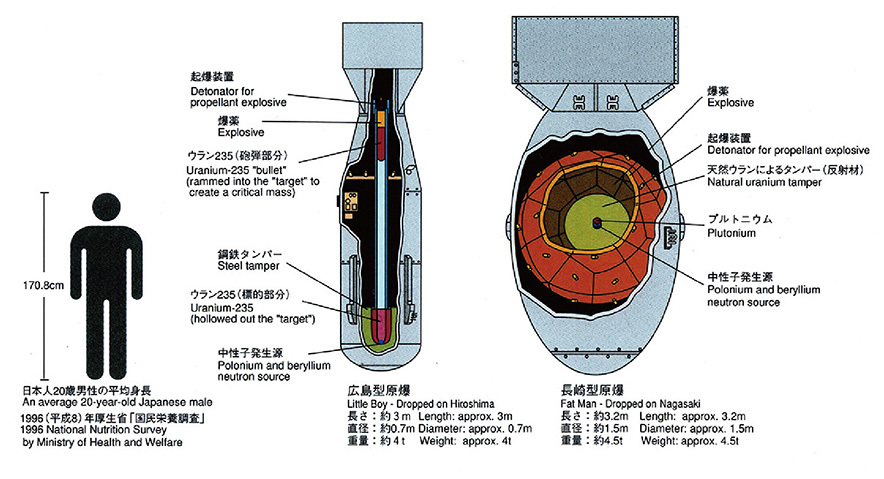
\includegraphics[width=0.62\textwidth]{Figures_History/Structure.jpg}
    \end{figure}
    \begin{itemize}
        \item 枪式构型:~\\
		{\fontsize{7.2pt}{6.2pt}\selectfont{把两块处于次临界状态的核材料,通过炸药爆炸产生的推力,使其迅速碰撞合并,达到超临界状态,进而引发链式反应。该方式核材料利用率低,现已较少使用}}
        \item 内爆式构型:~\\
		{\fontsize{7.2pt}{6.2pt}\selectfont{将核材料置于中心,周围包裹炸药。炸药起爆后,产生向心的冲击波,将核材料迅速压缩,使其达到超临界状态,引发链式反应。是较为经典的武器设计}}
    \end{itemize}
        将核材料、高精度的中子源、炸药以及复杂的引爆控制系统等部件,按照设计好的结构进行组装,确保各部件协同工作,实现核爆炸
%    \vspace{0.5cm}
%    \begin{figure}
 %       \includegraphics[width=0.8\textwidth]{uranium_mine.jpg}
%    \end{figure}
\end{frame}

% 幻灯片7:原子弹爆炸过程
%    \textbf{引爆过程}
\begin{frame}
    \frametitle{原子弹爆炸过程}
    \begin{enumerate}
		\setlength{\itemsep}{8pt}
	    \item 炸药起爆:~当接收到引爆指令,围绕核材料的炸药开始爆炸,产生强大的向心冲击波\\
		    {\fontsize{7.2pt}{6.2pt}\selectfont{以\textrm{TNT}炸药为例,爆速可达$6900\sim7100\mathrm{m/s}$,在极短时间内将能量传递给核材料}}
        \item 核材料压缩:~冲击波推动核材料迅速合拢,使其密度增加,体积减小,达到临界质量\\
		{\fontsize{7.2pt}{6.2pt}\selectfont{核材料中的中子引发核裂变的概率大幅提高}}
        \item 中子源启动:~高精度的中子源发射中子\\
		{\fontsize{7.2pt}{6.2pt}\selectfont{中子迅速轰击处于超临界状态的核材料,引发链式反应}}
        \item 能量释放:~核材料持续进行链式反应,在极短时间内释放出巨大的能量\\
		{\fontsize{7.2pt}{6.2pt}\selectfont{形成强烈的光辐射、高速运动的冲击波以及具有强穿透性的核辐射}}
    \end{enumerate}
\end{frame}

\begin{frame}
    \frametitle{原子弹爆炸过程}
    \vspace{-0.4cm}
    \begin{figure}
        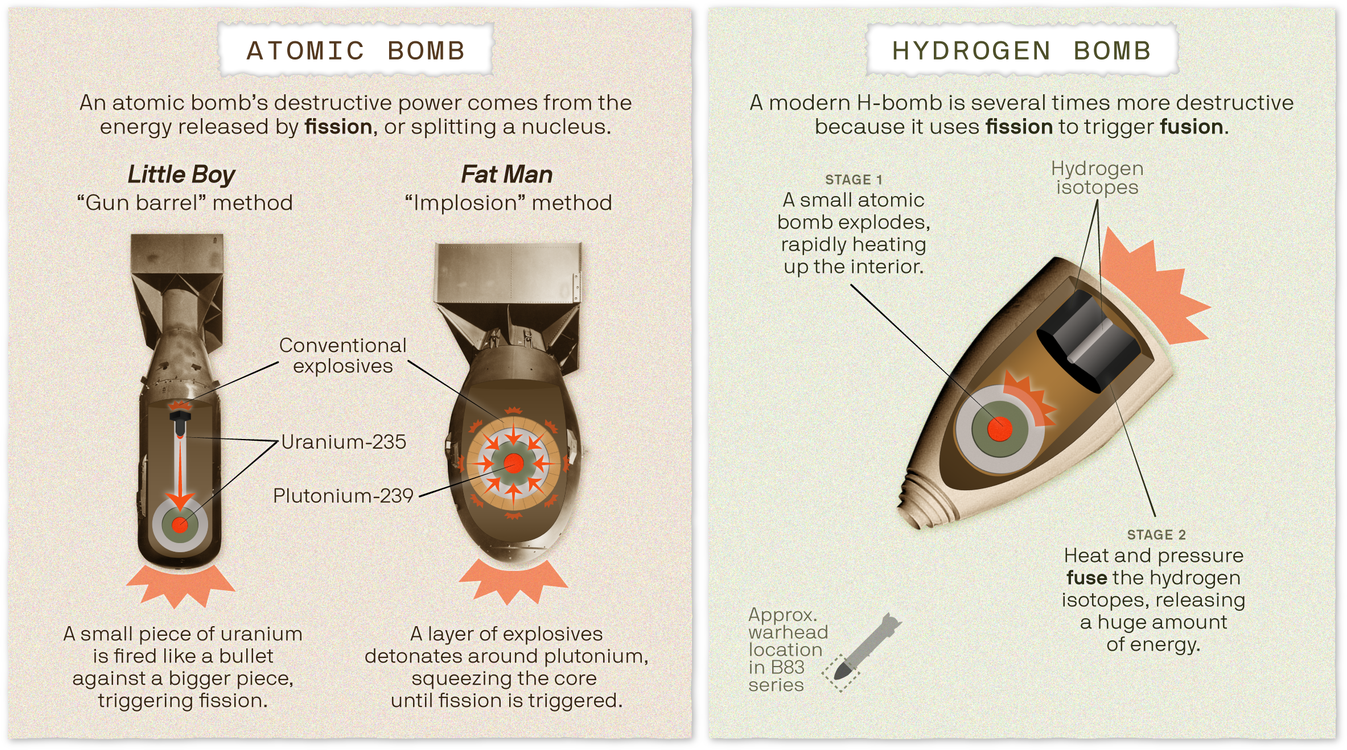
\includegraphics[width=0.7\textwidth,viewport=0 0 170 180,clip]{Figures_History/Nuclear_bomb.png}
    \end{figure}
\end{frame}

% 幻灯片8:聚变之光——氢弹原理
\section{氢弹的原理与引爆}
\begin{frame}
    \frametitle{聚变之光——氢弹原理}
%    \textbf{核聚变}
    \vspace{-0.4cm}
    \begin{figure}
       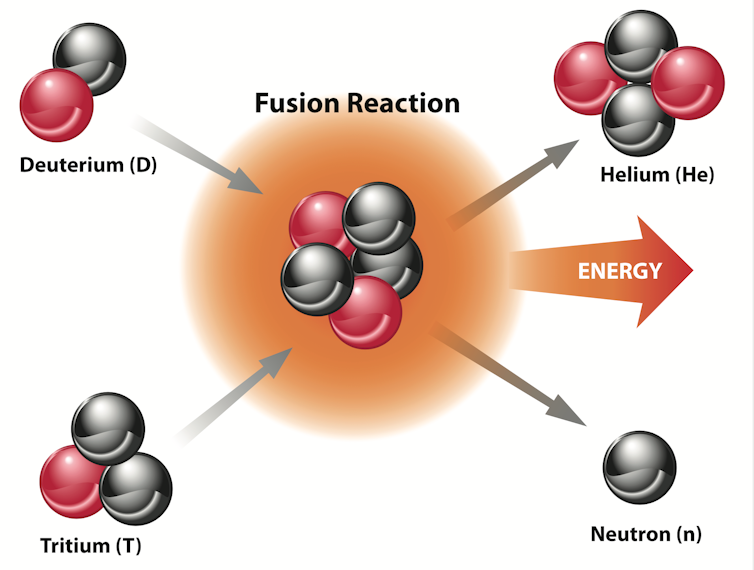
\includegraphics[width=0.5\textwidth]{Figures_History/Nuclear_Fusion.png}
    \end{figure}
    \begin{itemize}
        \item 聚变原理:\\
		{\fontsize{7.2pt}{6.2pt}\selectfont{氢的同位素氘($^2_1\mathrm{H}$)和氚($^3_1\mathrm{H}$)原子核,在数千万度乃至更高的超高温和超高压环境下,原子核具有足够动能克服斥力,合并成一个氦核($^4_2\mathrm{He}$),同时释放出一个中子和大量能量\\反应方程式可以表示为:
		\begin{displaymath}
			^2_1\mathrm{H} + ^3_1\mathrm{H} \rightarrow ^4_2\mathrm{He} + ^1_0n +\mathrm{Energy}
		\end{displaymath}}}
        \item 热核反应:~核聚变需要的在超高温、超高压条件下进行\\
		{\fontsize{7.2pt}{6.2pt}\selectfont{必须借助外界能量输入,营造出可使轻核发生聚变的极端环境}}
    \end{itemize}
\end{frame}

% 幻灯片9:氢弹材料制备
\begin{frame}
    \frametitle{氢弹材料制备}
    \begin{itemize}
	    \item 氘的获取:~氘在海水中以重水($\mathrm{D}_2\mathrm{O}$)的形式存在\\
		    {\fontsize{7.2pt}{6.2pt}\selectfont{海水中氘的含量约为氢的0.015\%,可通过电解法或蒸馏法,从重水中分离提取出氘}}
    \vspace{-0.2cm}
    \begin{figure}
        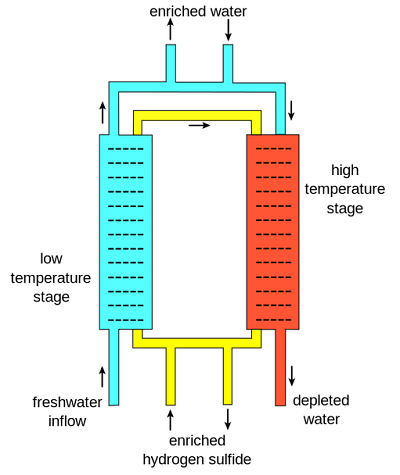
\includegraphics[width=0.3\textwidth]{Figures_History/Heavy_Water.png}
    \end{figure}
        \item 氚的生产:~氚具有放射性,半衰期约为12.3年,自然界中存量极少\\
		{\fontsize{7.2pt}{6.2pt}\selectfont{通常在核反应堆内,用中子辐照$^6\mathrm{Li}$来生产氚,反应式可表示为:
			\begin{displaymath}
				^6_3\mathrm{Li} + ^1_0n \rightarrow ^4_2\mathrm{He} + ^3_1\mathrm{H}
			\end{displaymath}}}
    \end{itemize}
%    \vspace{0.5cm}
%    \begin{figure}
        % 此处放置海水提取重水或核反应堆生产氚的示意图片
%        \caption{氢弹材料制备}
%    \end{figure}
\end{frame}

\begin{frame}
	\frametitle{氢弹的\textrm{Teller–Ulam}构型}
	美国的``\textrm{Teller–Ulam}''构型是世界上最早的氢弹构型\\
    \vspace{-0.3cm}
    \begin{figure}
        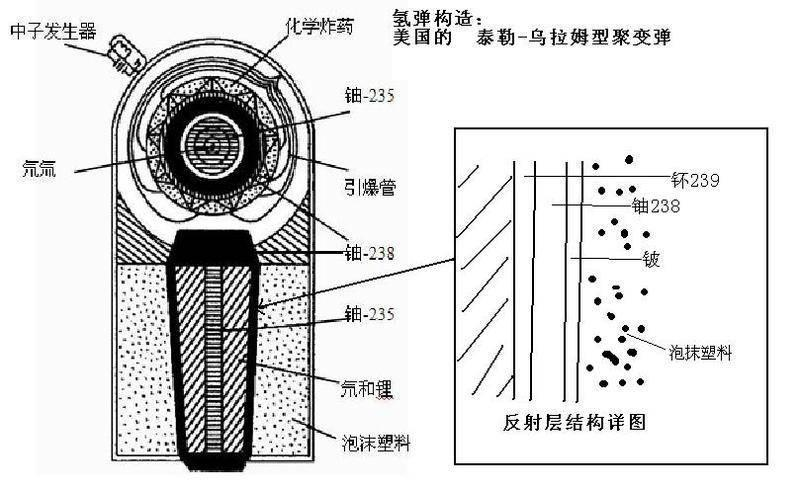
\includegraphics[width=0.8\textwidth]{Figures_History/U-T_design.jpg}
    \end{figure}
    ``\textrm{Teller–Ulam}''构型的氢弹采用两级炸弹结构,存在保存养护成本高、体积大等缺点
\end{frame}

\begin{frame}
    \frametitle{中国氢弹的核心突破}
    \textrm{20}世纪\textrm{60}年代,国际上对氢弹技术严密封锁,于敏、黄祖洽等科学家在艰难条件下,独立开展氢弹原理和构型的研究\\
    \begin{itemize}
	    \item \textcolor{red}{材料创新:}\\
		    {\fontsize{7.2pt}{6.2pt}\selectfont{使用固态氘化锂作为热核燃料,解决了传统液氚燃料储存和维护难题,极大提高了氢弹的稳定性和可靠性}}
	    \item \textcolor{red}{独特设计:}\\
		    {\fontsize{7.2pt}{6.2pt}\selectfont{我国氢弹的构型采用的物理设计,巧妙利用原子弹爆炸产生的辐射,更高效地压缩和点燃聚变材料,提升核聚变反应效率}}
	    \item \textcolor{red}{小型化优势:}\\
		    {\fontsize{7.2pt}{6.2pt}\selectfont{在同等当量下,我国氢弹的体积更小、重量更轻,便于搭载和投放,增强了武器的机动性和实用性}}
    \end{itemize}
    我国仅用2年8个月就成功完成从原子弹到氢弹的跨越,相比其他国家,大大缩短了研发时间
\end{frame}

\begin{frame}
    \frametitle{氢弹的引爆}
%    \textbf{引爆方式}
    氢弹需借助原子弹作为``扳机''来启动核聚变反应:
    \vspace{-0.1cm}
    \begin{figure}
        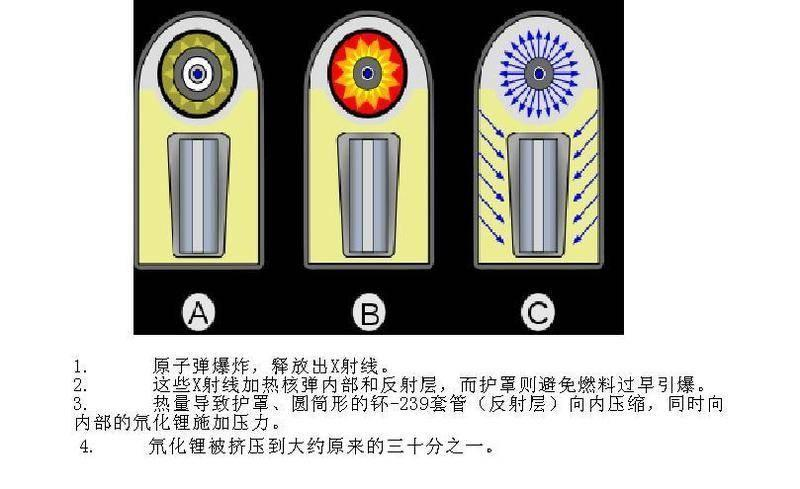
\includegraphics[width=1.0\textwidth]{Figures_History/U-T_design-2.jpg}
    \end{figure}
%    \begin{enumerate}
%        \item 原子弹引爆:\\
%		{\fontsize{7.2pt}{4.2pt}\selectfont{触发原子弹内的核裂变反应,释放出强烈的光辐射、\textrm{X}射线和高能粒子流}}
%        \item 辐射内爆:\\
%		{\fontsize{7.2pt}{4.2pt}\selectfont{强辐射与粒子流作用于氢弹的聚变材料,使其迅速升温、增压,形成向心的内爆过程,压缩聚变材料}}
%        \item 核聚变启动:\\
%		{\fontsize{7.2pt}{4.2pt}\selectfont{在超高温、超高压环境下,氢的同位素发生聚变反应,释放出更为巨大的能量,其威力通常远超作为``扳机''的原子弹}}
%    \end{enumerate}
\end{frame}

\begin{frame}
    \frametitle{战略核武器小型化}
重要意义
    \begin{itemize}
	    \item \textcolor{magenta}{提升机动性:}\\
		{\fontsize{6.2pt}{4.2pt}\selectfont{小型化的战略核武器,体积和重量大幅减小,可搭载于多种平台,如导弹、潜艇、战机等,显著增强了核力量的机动性与灵活性,能够实现快速部署与打击}}
	\item \textcolor{magenta}{增强突防能力}\\
		{\fontsize{6.2pt}{4.2pt}\selectfont{体积更小的核弹头,有助于降低被敌方探测和拦截的概率,提升核打击的有效性和可靠性}}
	\item \textcolor{magenta}{降低成本}\\
		{\fontsize{6.2pt}{4.2pt}\selectfont{减少核材料和其他组件的使用量,在保证核威慑力的同时,降低了研发、生产和维护成本}}
    \end{itemize}
%    \vspace{0.5cm}
实现途径
    \begin{itemize}
        \item 优化设计:\\
		{\fontsize{6.2pt}{4.2pt}\selectfont{通过改进核弹头的结构设计,%如采用更紧凑的核反应装置和更高效的引爆系统,在不降低爆炸威力的前提下,减小核弹头的体积和重量\\
		%以新型内爆式结构设计为例,能够更精准地控制核反应过程,
		提高核材料的利用率}}
        \item 新材料应用:\\
		{\fontsize{6.2pt}{4.2pt}\selectfont{研发和使用新型材料,%如高强度、低密度的结构材料,以及性能更优异的核材料,
		减轻核弹头的重量,提高其性能和可靠性}}
    \end{itemize}
%    \vspace{0.5cm}
%    \textbf{中国成就}
    我国在战略核武器小型化领域取得了显著成就,不仅提升了我国核力量的现代化水平,也为维护国家安全和世界和平做出了重要贡献
%    \vspace{0.5cm}
%    \begin{figure}
 %       %此处可插入中国小型化战略核武器或相关运载平台的示意图片
 %       \caption{中国小型化战略核武器成果}
 %   \end{figure}
\end{frame}

\section{``两弹一星''精神}
\begin{frame}
    \frametitle{``两弹一星''精神}
%    今天我们回顾了“两弹”的研发历程,认识了伟大的两弹元勋,探索了原子弹和氢弹背后的科学原理,领略了于敏构型的独特魅力,以及战略核武器小型化的成就。“两弹”精神将激励我们为中华民族伟大复兴不懈奋斗!
    {\centering{\huge\textcolor{red}{
	    热爱祖国、无私奉献\\
    自力更生、艰苦奋斗\\
    大力协同、勇于登攀\\}}}
%    \vspace{-0.05cm}
    \begin{figure}
        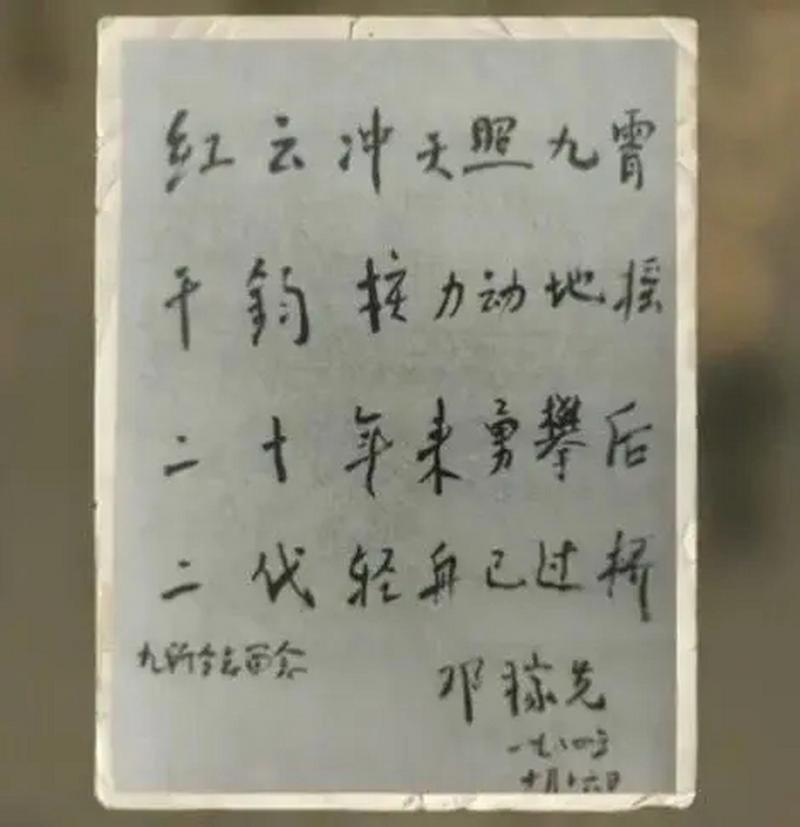
\includegraphics[height=0.4\textwidth]{Figures_History/Deng_Jiaxian.jpeg}
        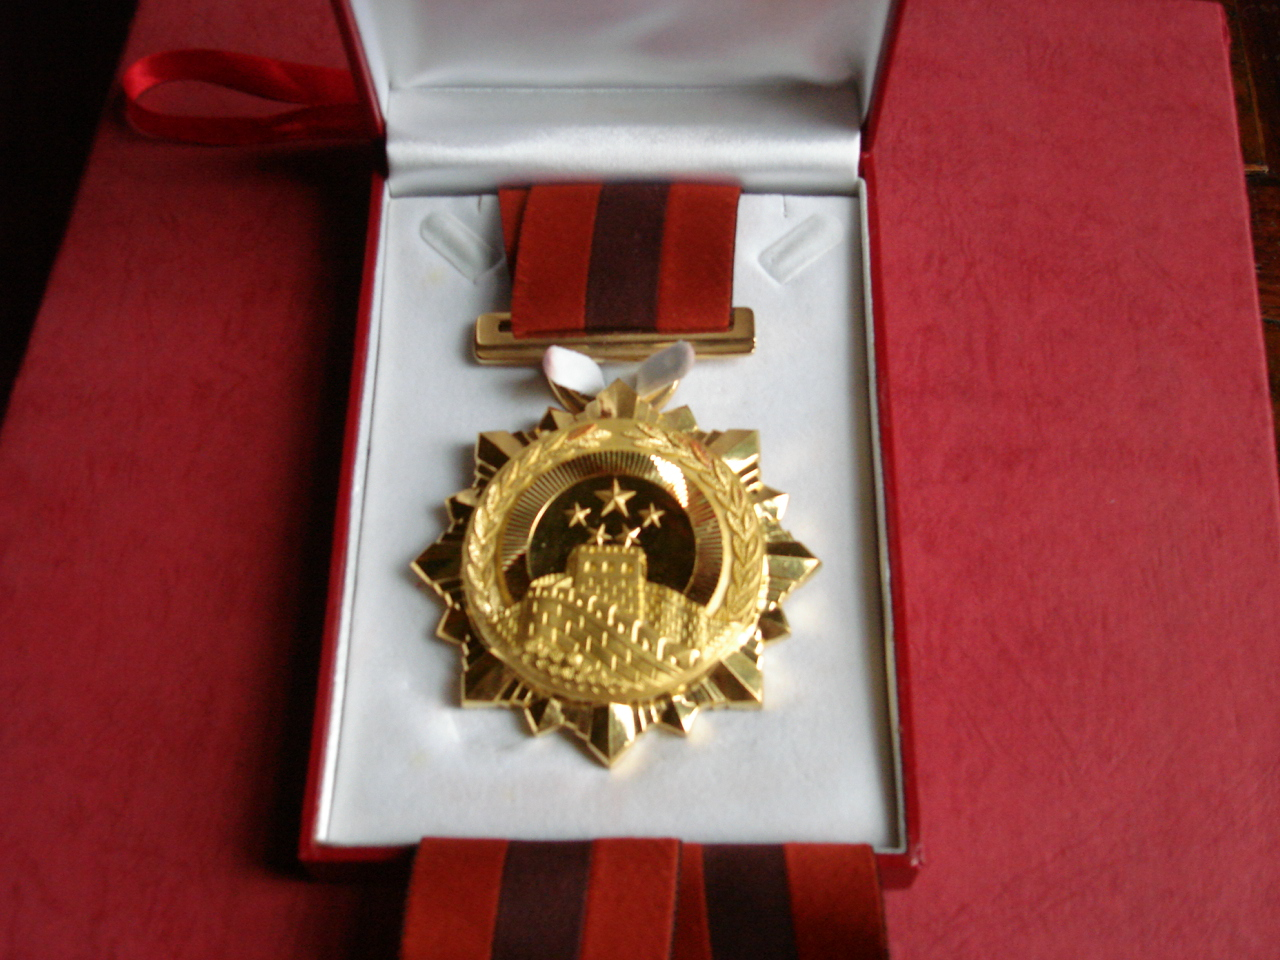
\includegraphics[height=0.4\textwidth]{Figures_History/Ward_for_Peng-Huanwu.jpg}
    \end{figure}
\end{frame}
